\chapter{Socio-economic environment}\label{ch:socio_economic_environment}

The widespread adoption of \glspl{uav} is transforming society and the economy, offering significant benefits while also presenting challenges. This chapter examines the socio-economic factors influencing the deployment of autonomous drones, particularly in \glspl{ntn} for remote areas. It explores the potential advantages, obstacles, and financial implications of integrating this technology across industries.

\section{Social Impact}\label{sec:social_impact}

Autonomous \glspl{uav} have gained popularity due to their versatility and efficiency, revolutionizing fields like agriculture, construction, and public safety. Their ability to perform complex tasks quickly can greatly enhance societal well-being. For example, \glspl{uav} equipped with thermal cameras improve emergency response by locating individuals in burning buildings, while high-resolution cameras can monitor large events. The project demonstrated how \glspl{uav} can provide real-time reconnaissance, aiding first responders and improving public safety.

In remote regions, autonomous \glspl{uav} facilitate connectivity by delivering essential supplies such as medicine and food. This capability not only improves the quality of life but also bridges the digital divide by providing internet access to underserved communities, thereby enhancing educational and informational resources.

However, privacy and security remain concerns. The extensive data collection by \glspl{uav} raises issues of surveillance, while the potential for misuse, such as spying or attacks, underscores the need for clear regulations and ethical guidelines, see \cref{ch:regulatory_framework}.

\section{Economic Impact}\label{sec:economic_impact}

The economic benefits of adopting autonomous \glspl{uav} are substantial, with the potential to boost productivity and drive innovation. In agriculture, \glspl{uav} enable precision farming through crop monitoring, pest detection, and optimized irrigation, helping farmers improve yields and reduce costs. The construction industry also benefits, as \glspl{uav} offer efficient infrastructure inspections, reducing manual labor and associated risks.

Despite these advantages, the costs of adopting \glspl{uav} (e.g., purchase, training, maintenance, and insurance) remain significant barriers for small companies and groups. Moreover, the need for skilled operators and the risk of accidents or malfunctions can increase operational expenses which is specially challenging for research groups in \glspl{ntn}.

\section{Environmental Impact}\label{sec:environmental_impact}

Autonomous \glspl{uav} can positively impact the environment by reducing fossil fuel usage. Their electric motors are more energy-efficient and produce fewer emissions than traditional vehicles, contributing to lower air pollution and greenhouse gas levels.

Nonetheless, the environmental costs of manufacturing and disposing of \glspl{uav} must be considered. The production of lightweight materials like carbon fiber is energy-intensive, and lithium-ion batteries pose recycling challenges. Sustainable design practices are necessary to mitigate these effects.

\section{Project Planning}

The project was structured into distinct phases, each with specific activities and tasks, as illustrated in \cref{fig:planning}. The timeline for these phases was planned on a weekly basis, detailing the progression of activities from initial research to final flight tests. The first month and a half of the project was dedicated to understanding the problem, reviewing relevant literature, exploring the necessary tools, and configuring them for our specific needs. This initial phase, encompassing research and planning, required a significant time investment due to the complexities and documentation gaps associated with certain tools like Mission Planner or hardware integration. The subsequent five months were focused on building of the UAV and the development of the system and the final three months to writing the final document.

\begin{figure}
    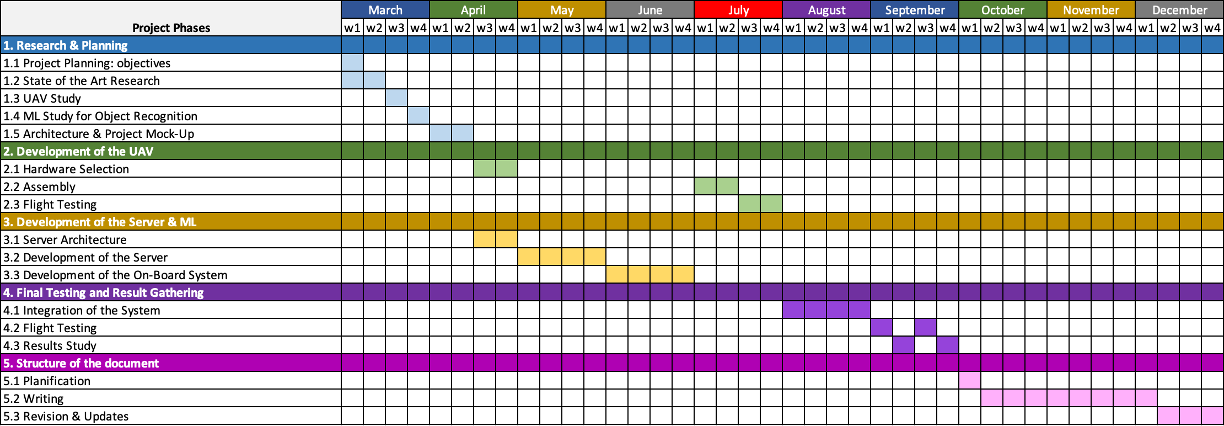
\includegraphics{planning.png}
    \caption{Gantt Chart for the Project Planning}\label{fig:planning}
\end{figure}

\section{Project Budget}\label{sec:budget_analysis}

As previously mentioned, the cost of adopting autonomous drones is a significant hurdle. This section breaks down the expenses associated with purchasing and operating drones, categorized into manufacturing, operating, and additional costs. The analysis includes a detailed assessment of hardware components, maintenance, insurance, and other relevant expenses.

Tables \cref{tab:manufacturing_costs_uav}, \cref{tab:manufacturing_costs_reconnaissance_platform}, \cref{tab:operating_costs}, \cref{tab:other_costs}, and \cref{tab:human_costs} provide comprehensive cost breakdowns. The total cost, encompassing all categories, offers a clear picture of the financial investment needed for adopting drones in \glspl{ntn} applications. For this project, the total cost amounts to 20216 \euro, which includes the necessary hardware, software, development, and operational expenses. However, it does not account for maintenance costs, such as training and operator salaries, which are essential for long-term sustainability.

In conclusion, while autonomous drones hold significant promise for remote areas and various industries, careful consideration of social, economic, and environmental factors is essential. Addressing these challenges with appropriate regulations and sustainable practices will maximize their potential benefits.

\begin{table}[H]
  \begin{tabular}{ l l r r }
    \toprule
    \textbf{Item} & \textbf{Model} & \textbf{Quantity} & \textbf{Cost (\euro)} \\
    \midrule
    Airframe & Tarot XS690 \autocite{rcinnovationsQuadPlegable} & 1 & 199 \\
    Motors & Tmotor U7 V2 420KV \autocite{rcinnovationsTmotor420KV} & 4 & 520 \\
    \gls{esc} & Tmotor FLAME 100A LV 600Hz \autocite{rcinnovationsVariadorTmotor} & 4 & 360 \\
    Propellers & Tmotor 17$\times$5.8 V2 \autocite{rcinnovationsTmotor17x58} & 2 & 144 \\
    Flight Controller & Holybro Pixhawk 6C \autocite{rcinnovationsPixhawkCarcasa} & 1 & 207 \\
    Battery & TATTU 22000mAh 4S 14.8V 30C \autocite{rcinnovationsComprarBatera}  & 1 & 270 \\
    \gls{pdb} & Holybro PM07 Power Module \autocite{rcinnovationsHolybroPM07} & 1 & 48 \\
    Regulator & HobbyWing 25A HV UBEC \autocite{rcinnovationsHobbyWingUbec} & 1 & 58 \\
    \gls{gps} & Holybro M9N GPS GNSS \autocite{rcinnovationsHolybroGNSS} & 1 & 70 \\
    Radiocontroller & RadioMaster TX16S \autocite{rcinnovationsRadioMasterTX16S} & 1 & 200 \\
    \gls{rf} Module & RFD868 TXMOD V2 868Mhz 1W \autocite{rcinnovationsComprarMdulos} & 1 & 423 \\
    Miscellaneous & Screws, Nuts, Wires, etc. &~--~& 100 \\
    \midrule
    \textbf{Total} & & & 2599 \\
    \bottomrule
  \end{tabular}
  \caption{Manufacturing costs for the \gls{uav}.}\label{tab:manufacturing_costs_uav}
\end{table}

\begin{table}[H]
  \begin{tabular}{ l l l r }
    \toprule
    \textbf{Item} & \textbf{Model} & \textbf{Quantity} & \textbf{Cost (\euro)} \\
    \midrule
    On-board Computer & NVIDIA Jetson Orin \autocite{nvidiaNVIDIAJetson} & 1 & 831 \\
    Camera & Ricoh Theta X 360 Degree Camera \autocite{ricohimagingTHETARicoh} & 1 & 800 \\
    Router & GL.iNet GL-X750 \autocite{glinetGLX750Spitz} & 1 & 153  \\
    4G SIM Card & Orange Prepaid SIM Card (1 month) & 1 & 10 \\
    Server & Amazon Web Services (1 month) & 1 & 10 \\
    \midrule
    \textbf{Total} & & & 1804 \\
    \bottomrule
  \end{tabular}
  \caption{Manufacturing costs for the reconnaissance platform} \label{tab:manufacturing_costs_reconnaissance_platform}
\end{table}

\begin{table}[H]
    \begin{tabular}{ l l r }
        \toprule
        \textbf{Item} & \textbf{Description} & \textbf{Cost (\euro)} \\
        \midrule
        Insurance & Liability Insurance for Pilots & 50 \\
        Flying Field & Flying Club Membership (1 year) & 350 \\
        Licensing & Drone Pilot License (1 year) & 0 \\
        Software & ArduPilot Software License (1 year) & 0 \\
        Maintenance & Spare Parts & 50 \\
        \midrule
        \textbf{Total} & & 450 \\
        \bottomrule
    \end{tabular}
    \caption{Operating costs.}\label{tab:operating_costs}
\end{table}

\begin{table}[H]
    \begin{tabular}{ l l r r }
        \toprule
        \textbf{Item} & \textbf{Model} & \textbf{Quantity} & \textbf{Cost (\euro)} \\
        \midrule
        Battery Charger & ISDT K4 Dual Charger \autocite{rcinnovationsISDTCargador} & 1 & 200 \\
        Lipo Bags & Lipo Safe Bags (Large) \autocite{rcinnovationsBolsaProtectora} & 1 & 13 \\
        Tools & Screwdriver Set, Pliers, etc. &~--~& 50 \\
        Solders & Soldering Iron, Solder, etc. &~--~& 200 \\
        3D Printer & Bamboo P1S \autocite{bambulabBambuPrinter} & 1 & 1015 \\
        3D Filament & PLA Filament (1kg) & 1 & 30 \\
        \midrule
        \textbf{Total} & & & 1508 \\
        \bottomrule
    \end{tabular}
    \caption{Other costs.}\label{tab:other_costs}
\end{table}

\begin{table}[H]
    \begin{tabular}{ l l l r }
        \toprule
		\textbf{Item}  & \textbf{Model}                           & \textbf{Quantity} & \textbf{Cost (\euro)} \\
        \midrule
        Personal Computer & Macbook Air & 1 & 1600  \\
        Junior Engineer Hours & 15 \euro/h & 500 & 7500 \\
        Senior Engineer Hours & 60 \euro/h & 40 & 2400 \\
        Electricity, labs, climate control, management, etc. & & & 2040 \\
        \midrule
        \textbf{Total} & & & 13900 \\
        \bottomrule
    \end{tabular}
    \caption{Human costs.}\label{tab:human_costs}
\end{table}
